\chapter*{Resultados}
Como resultado del proceso de acompañamiento con el laboratorio de creación se crearon una serie de mockups que sirvieron para comprender a grandes rasgos el funcionamiento de la nueva plataforma, estos mockups se presentan en los anexos del 1 al 4. Ademas los formatos diligenciados de cada sesión se pueden encontrar en la siguiente dirección \url{https://goo.gl/ZujiKj} donde se puede observar el proceso de concepción del problema a solucionar con la nueva plataforma, las acciones necesarias a seguir y por ultimo el desarrollo y sostenibilidad de la marca.\\

Luego de definir la metodología de desarrollo se procedió a construir los requisitos iniciales de la plataforma los cuales se registraron utilizando la herramienta Enterprise Architect los cuales comprenden los módulos de registro de actores y de dashboard de administración (Ver figuras 4 y 5)\\ 

\begin{figure}[ht]
	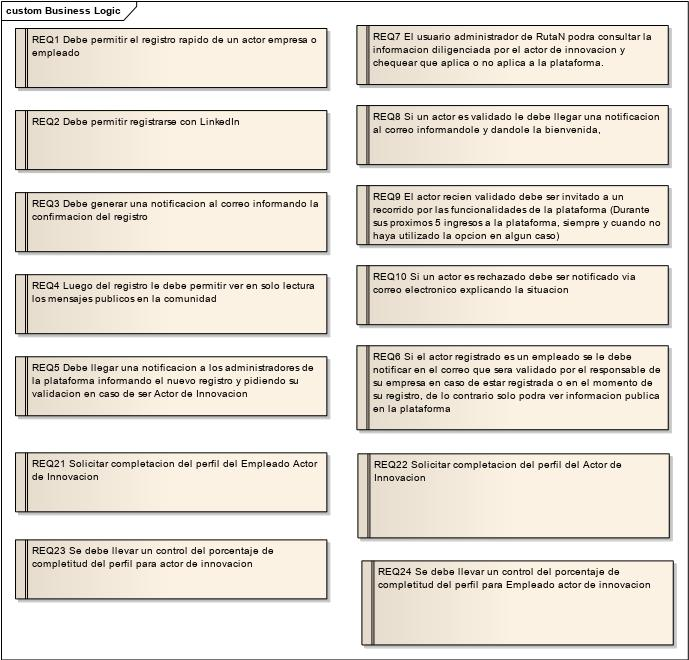
\includegraphics[scale=0.6, center]{images/registro.jpg}
	\caption{Historias de usuario referentes al registro de actores}
	\label{fig:img4}
\end{figure}

\begin{figure}[ht]
	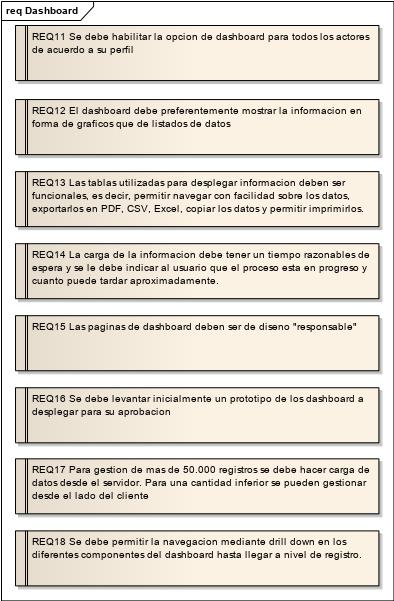
\includegraphics[scale=0.6, center]{images/dashboard.jpg}
	\caption{Historias de usuario referentes al dashboard de administración}
	\label{fig:img5}
\end{figure}

Estos requisitos se formularon en base a unos objetivos organizacionales que posee la
corporación, por lo anterior fue necesario identificar los objetivos de negocio y presentarlos
mediante una serie de casos de uso del negocio y su relación con los respectivos actores de
la plataforma (ver figura 6).\\

\begin{figure}[ht]
	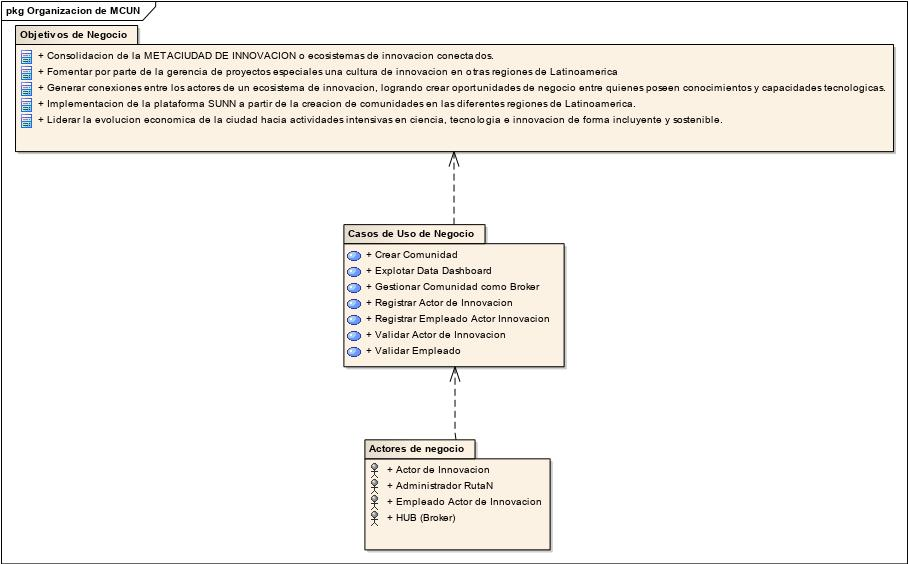
\includegraphics[scale=0.6, center]{images/negocio.jpg}
	\caption{Relación entre los objetivos de negocio con los actores de la platafoma}
	\label{fig:img6}
\end{figure}

En la figura 7 se describen las relaciones de cada actor del negocio con los casos
de uso del negocio y la interacción con otros actores de la plataforma que para el proyecto se
denominarán actores de innovación.\\

Si bien el Broker es un actor de innovación, en los diagramas se presenta como un actor por
separado ya que puede realizar unas acciones de mayor nivel que los demás, por otro lado,
también posee funciones de administración ya que coordina su propia comunidad compuesta
por una cantidad definida (por una licencia) de actores de innovación.\\

Por ultimo también se diferencia el actor empleado ya que en esta nueva versión de la
plataforma se permitirá el registro ilimitado de empleados de las empresas registradas, los
cuales tendrán la posibilidad de compartir contenidos en una sección Timeline tipo muro,
pero solo un empleado estará en la capacidad de administrar la empresa a la que pertenece,
generar conexiones con  los demás actores y aprobar o rechazar nuevos registros de
empleados que digan pertenecer a su empresa.\\


\begin{figure}[ht]
	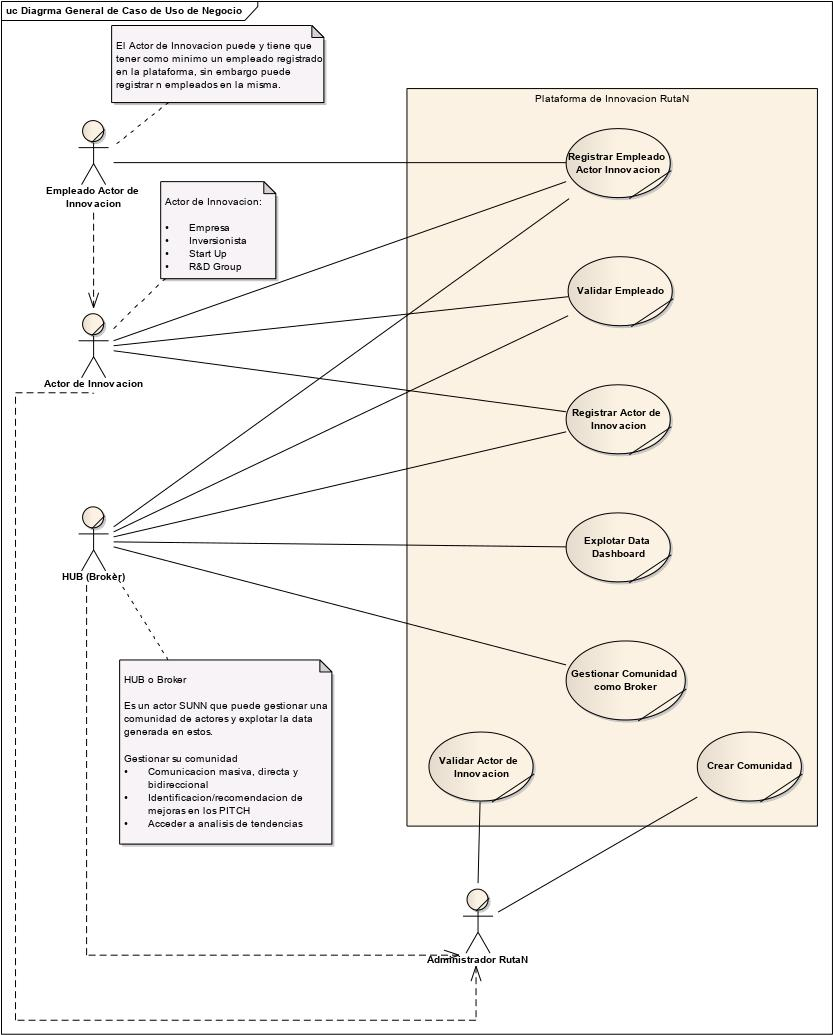
\includegraphics[scale=0.6, center]{images/casos.jpg}
	\caption{Diagrama de casos de uso general del negocio.}
	\label{fig:img7}
\end{figure}

Posteriormente con el fin de realizar la lógica necesaria para el dashboard de administración se realizó una tarea de estudio sobre esta misma funcionalidad en la plataforma antigua para comprender su funcionamiento, tarea que hasta ese momento no había sido realizada, al realizar el estudio se construyó un informe especificando el funcionamiento del modulo y su comportamiento que se describe por 4 métricas principales: Actividad, Atractividad, Visibilidad y Global Performance.\\

Cada una de las métricas se compone de uno o más parámetros, los cuales pueden ser:

\begin{itemize}
	\item SCOUTING: Tasa de apariciones de una empresa en el radar, se calcula de la siguiente manera
	\begin{itemize}
		\item nScouting = Numero de ocurrencias por células y región, al filtrar por célula y región se obtiene la cantidad de empresas  que pueden visualizar a la compañía a la que se le quiere calcular este parámetro.
		\item nCompanies = Numero total de empresas.
	\end{itemize}
	$Valor = nScouting/nCompanies$
	
	\item PROFILE\_PROGRESS: Tasa de completitud del perfil de usuario:
	
	\begin{itemize}
		\item nCompleted = Numero de campos completos.
		\item nTotal = Numero total de campos.
	\end{itemize}
	
	$Valor = nCompleted/nTotal$
	
	\item PROPOSED\_CHALLENGES: Numero de retos creados por la compañía.
	
	\item PROFILE\_VIEWS: Numero de visitas al perfil de una empresa en el ultimo año.
	
	\item RECEIVED\_WORKFLOWS: Numero de invitaciones a conectar recibidas por la compañía y aceptadas en el ultimo año.
	
	\item INITIATED\_WORKFLOWS: Numero de invitaciones a conectar enviadas por la compañía y aceptadas por la otra compañía en el ultimo año.
	
	\item INNOBOX: Numero de mensajes que ha recibido la compañía en el ultimo año.
	
\end{itemize}

En el cuadro 3 se observan los parámetros que se utilizan para calcular cada métrica y sus correspondientes pesos y limite máximo (el limite mínimo siempre es cero). Aunque el parámetro INNOSENSOR está presente en la tabla, en la funcionalidad de la plataforma se encuentra deshabilitado, por lo tanto no aporta valor a su métrica. \\

\begin{table}[ht]
	\centering
	\caption{Métricas del dashboard con sus parámetros}
	\label{table3}
	\begin{tabular}{|c|l|c|c|}
		\hline
		\textbf{Métrica} & \multicolumn{1}{c|}{\textbf{Parámetros}} & \textbf{Peso} & \multicolumn{1}{l|}{\textbf{Maximo}} \\ \hline
		{\textbf{Atractividad}} & PROFILE\_VIEWS & 0.2 & 15 \\ \cline{2-4} 
		& INNOBOX & 0.3 & 5 \\ \cline{2-4} 
		& RECEIVED\_WORKFLOWS & 1 & 2 \\ \cline{2-4} 
		& PROPOSED\_CHALLENGES & 0.1 & 5 \\ \hline
		{\textbf{Actividad}} & PROFILE\_PROGRESS & 0.15 & 1 \\ \cline{2-4} 
		& INITIATED\_WORKFLOWS & 0.8 & 3 \\ \cline{2-4} 
		& PROPOSED\_CHALLENGES & 0.05 & 5 \\ \hline
		{\textbf{Visibilidad}} & PROFILE\_VIEWS & 1 & 15 \\ \cline{2-4} 
		& SCOUTING & 0.7 & 1 \\ \cline{2-4} 
		& INNOSENSOR & 0.3 & 1 \\ \hline
	\end{tabular}
\end{table}

Ahora para calcular el valor de cada métrica, cada uno de sus parámetros debe pasar por el siguiente proceso:

\begin{enumerate}
	\item Se extrae el valor del parámetro como se indicó anteriormente
	\item Este valor pasa por un proceso de normalización donde:
	
	\begin{enumerate}
		\item si el valor es inferior a su limite mínimo, el valor se reemplaza por el limite mínimo.
		\item Si el valor es superior a su limite máximo, se reemplaza por el limite máximo.
		\item En otro caso el valor se reemplaza por la siguiente formula: \\\\
		$valor=\frac{valor - minimo}{maximo - minimo}$
	\end{enumerate}

	\item Luego de obtener los valores de los parámetros, se realiza un promedio ponderado multiplicando cada valor con su respectivo peso y se divide por el peso total de la siguiente manera: \\\\
	$\frac{\sum_{n = 1}^{\# parametros} valor_{n} * peso_{n}}{pesoTotal}$
	
	\item Por ultimo, para obtener el valor del Gobal Performance, se realiza un promedio simple entre las 3 métricas anteriores.
\end{enumerate}

Para obtener las métricas de administrador, se realiza un promedio de cada métrica con respecto a la cantidad de empresas que componen la comunidad del administrador.\\

Luego de realizar los cálculos de las métricas, las empresas son clasificadas en varios rangos, D menos, D, D más, C menos, C, C más, B menos, B, B más, A menos, A y A más. Los valores que toma la plataforma para clasificar a las compañías son: 

\begin{itemize}
	\item Si 0 <= actividad y atractividad < 0.166666667 entonces la empresa se clasifica en D menos
	\item Si 0.166666667 <= actividad < 0.333333333 y 0 <= atractividad < 0.333333333 entonces la empresa se clasifica en D
	\item Si 0 <= actividad < 0.333333333 y 0.166666667 <= atractividad < 0.333333333 entonces la empresa se clasifica en D
	\item Si 0.333333333 <= actividad < 0.5 y 0 <= atractividad < 0.5 entonces la empresa se clasifica en D mas
	\item Si 0 <= actividad < 0.5 y 0.333333333 <= atractividad < 0.5 entonces la empresa se clasifica en D mas
	\item Si 0.5 <= actividad < 0.666666667 y 0 <= atractividad < 0.166666667 entonces la empresa se clasifica en C menos
	\item Si 0.666666667 <= actividad < 0.833333334 y 0 <= atractividad < 0.333333333 entonces la empresa se clasifica en C
	\item Si 0.5 <= actividad < 0.833333334 y 0.166666667 <= atractividad < 0.333333333 entonces la empresa se clasifica en C
	\item Si 0.833333334 <= actividad < 1 y 0 <= atractividad < 0.5 entonces la empresa se clasifica en C mas
	\item Si 0.5 <= actividad < 1 y 0.333333333 <= atractividad < 0.5 entonces la empresa se clasifica en C mas
	\item Si 0 <= actividad < 0.166666667 y 0.5 <= atractividad < 0.666666667 entonces la empresa se clasifica en B menos
	\item Si 0.166666667 <= actividad < 0.333333333 y 0.5 <= atractividad < 0.833333334 entonces la empresa se clasifica en B
	\item Si 0 <= actividad < 0.333333333 y 0.666666667 <= atractividad < 0.833333334 entonces la empresa se clasifica en B
	\item Si 0.333333333 <= actividad < 0.5 y 0.5 <= atractividad < 1 entonces la empresa se clasifica en B mas
	\item Si 0 <= actividad < 0.5 y 0.833333334 <= atractividad < 1 entonces la empresa se clasifica en B mas
	\item Si 0.5 <= actividad < 0.666666667 y 0.5 <= atractividad < 0.666666667 entonces la empresa se clasifica en A menos
	\item Si 0.666666667 <= actividad < 0.833333334 y 0.5 <= atractividad < 0.833333334 entonces la empresa se clasifica en A
	\item Si 0.5 <= actividad < 0.833333334 y 0.666666667 <= atractividad < 0.833333334 entonces la empresa se clasifica en A
	\item Si 0.833333334 <= actividad < 1 y 0.5 <= atractividad < 1 entonces la empresa se clasifica en A mas
	\item Si 0.5 <= actividad < 1 y 0.833333334 <= atractividad < 1 entonces la empresa se clasifica en A mas
\end{itemize}


